\section{Residue Calculus}
Evaluating integrals by way of computing residues can allow us to compute certain integral that would difficult, or in some case impossible, by the usual methods of integration (i.e finding primitives).
\subsection{Rational functions of sin and cos}
Suppose $R(x, y)$ is a (real) rational function (in two coordinates) with no poles on the unit circle and we wish to evaluate
$$ \int_0^{2\pi} R(\cos \theta, \sin \theta) d\theta $$
In principle, we could handle this by usual methods of integration and residue calculus is not strictly required. However, we will see that this makes the task a lot easier.

First note that since we are integrating on the unit circle, we can substitute $z = e^{i \theta}$. Then we can write $\cos \theta$ and $\sin \theta$ in terms of $z$ and $z^{-1}$.
\begin{align*}
    \int_0^{2\pi} R(\cos \theta, \sin \theta) d\theta &= -i \int_{\abs{z} = 1} R \left( \frac{1}{2} \left(z + \frac{1}{z}\right), \frac{1}{2i} \left(z - \frac{1}{z}\right)    \right) \frac{dz}{z} = 2\pi \sum_{\abs{z} < 1} res \left( g(z) \right)
\end{align*}
where 
$$ g(z) = \frac{1}{z}R \left( \frac{1}{2} \left(z + \frac{1}{z}\right), \frac{1}{2i} \left(z - \frac{1}{z}\right) \right) $$
The sum is actually a sum over the residue of the poles of $g$ that lie inside the unit disk (in other words we are exactly applying the Residue Theorem). Such notation will be consistently used in this section.

For a concrete example, suppose we want to compute
$$\int_0^\pi \frac{d\theta}{a + \cos \theta}$$
where $a > 1$ is a real number.
We cannot apply the procedure above directly since we are integrating from $0$ to $\pi$ instead of $0$ to $2\pi$ (so in other words when we interpret this integral in the complex plane we don't actually form a closed curve). However, since $\cos(\theta) = \cos(2 \pi - \theta)$ we get that 
$$\int_0^\pi \frac{d\theta}{a + \cos \theta} = \int_\pi^{2\pi} \frac{d\theta}{a + \cos \theta}$$
and therefore
$$\int_0^\pi \frac{d\theta}{a + \cos \theta} = \frac{1}{2}\int_0^{2\pi} \frac{d\theta}{a + \cos \theta}$$
The integral on the right hand side can be compute as above. We substitute $z = e^{i \theta}$ giving us 
\begin{align*}
    \int_0^{2\pi} \frac{d\theta}{a + \cos \theta} &= -i \int_{\gamma} \frac{1}{a + \frac{1}{2}\left(z + \frac{1}{z} \right)} \cdot \frac{dz}{z}\\
    &= -2i \int_{\gamma} \frac{1}{z^2 + 2az + 1} dz
\end{align*}
where $\gamma$ is the unit circle oriented positively. As mentioned, we will use the Residue Theorem to calculate this. For this we need to know the poles of the rational function in the integrand that lie in the unit disk. The poles of the integrand are exactly the zeroes of $z^2 + 2az + 1$ which are $-a \pm \sqrt{a^2 - 1}$. Since we assumed $a$ to be real and greater than 1, it is clear that both roots are real. However, only one of them lies inside the unit disk, namely $-a + \sqrt{a^2 - 1}$. 

Therefore we need to compute the residue of the integrand at $-a + \sqrt{a^2 - 1}$. We see that this is a simple pole (there are only 2 poles and the other pole is obviously distinct). This makes it easy to compute the residue to be
$$ \frac{1}{2(z + a)} \bigg|_{z = -a + \sqrt{a^2 - 1}} = \frac{1}{2\sqrt{a^2 - 1}} $$
(see \autoref{eg:residue-of-quotient}). Therefore by the Residue Theorem
$$ \int_\gamma \frac{1}{z^2 + 2az + 1}dz = 2\pi i \cdot \frac{1}{2\sqrt{a^2 - 1}} $$
Therefore 
$$ \int_0^\pi \frac{d\theta}{a + \cos \theta} = \frac{1}{2} \cdot -2i \cdot \frac{2\pi i}{2\sqrt{a^2 - 1}} = \frac{\pi}{\sqrt{a^2 - 1}}$$

\subsection{Rational functions over the real line}
Suppose $R(x)$ is a rational function with no real poles and we wish to compute
$$\int_{-\infty}^{\infty} R(x) dx$$
Recall that this integral is defined to be
$$\int_{-\infty}^0 R(x) dx + \int_0^{\infty} R(x) dx$$
Thus the integral over the real line exists if and only if both of the integrals in the sum above exist. These integrals exist if and only if $R$ has zeros of (at least) order 2 at $\infty$ and $-\infty$. This is equivalent to saying that 
$$\lim_{x \to \pm \infty} xR(x) = 0$$

In order to evaluate this integral we will evaluate over a certain curve in the complex plane that includes a part of the real line. We will see that the portion of the curve that does not lie on the real axis contributes negligibly to the integral, especially when we consider larger and larger curves. Hence, the value of the integral over the entire curve is very well approximated by the value of the integral over the real line and in the limit the two are equal. On the other hand, the integral over the entire curve can be calculated easily by the Residue Theorem. Hence this gives us a fairly easy way to compute the integral of the rational function over the entire real line.

\begin{figure}[h]
    \centering
    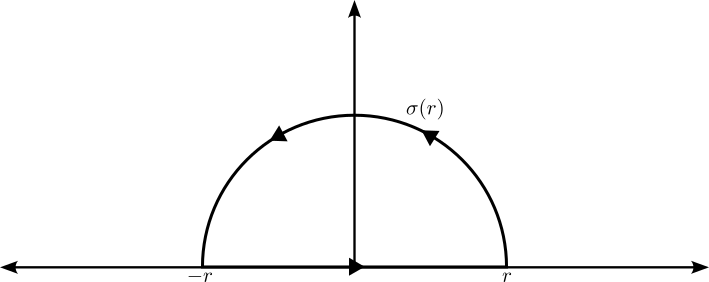
\includegraphics{Images/real_line_contour.png}
    \caption{We integrate over a semicircle in the (closed) upper half-plane}
    \label{fig:real-line-contour}
\end{figure}

Now, to make the above outline more precise. Let $\gamma(r)$ be a semicircle in the upper half-plane centered at 0 and of radius $r$ (including the diameter formed by the interval $[-r, r]$). Let $\sigma(r)$ denote the circular arc itself (not including $[-r, r]$) so that $\gamma(r) = \sigma(r) + [-r, r]$. 
If we take $r$ large enough then all the poles of $R$ that are in the upper half-plane are inside $\gamma(r)$. Then we get 
$$\int_{\gamma(r)} R(z) dz = \int_{-r}^r R(x) dx + \int_{\sigma(r)} R(z) dz = 2\pi i \sum_{\Im(z) > 0} res(R(z))$$
I claim that as $r \to \infty$, the integral over $\sigma(r)$ goes to 0 which would imply that
$$\int_{-\infty}^\infty R(x) dx = 2\pi i \sum_{\Im(z) > 0} res(R(z))$$

In order to see that the claim holds let $M(r)$ be the supremum of $R(re^{i \theta})$ for $\theta \in [0, \pi]$. Then
$$ \int_{\sigma(r)} R(z) dz \leq M(r) \int_{\sigma(r)} dz = M(r) \cdot -2r $$
Since we know that $zR(z) \to 0$ as $z \to \infty$ we conclude that the above integral goes to 0 as $r \to \infty$. 

Note that we could also integrate in the lower half-plane if we so wished by simply reflecting the contour across the real axis. However in order to integrate along the real axis in the usual direction we would need to consider this contour with a negative orientation.\\

For a concrete example, we compute
$$ \int_0^{\infty} \frac{dx}{1 + x^6} $$
Again the integral is over the non-negative reals instead over the entire real line as we calculated above but we will do the same thing as before by computing half the integral over the entire real line (note that the integrand is even).

We see that $\frac{1}{1 + z^6}$ has 6 poles, all of which lie on the unit circle. There are 3 poles that lie in the upper half-plane: $e^{\pi i/6}, e^{\pi i/2}$ and $e^{5\pi i/6}$. The residue at each pole $\alpha$ is
$$ \frac{1}{6\alpha^5} = \frac{-\alpha}{6} $$
where we use the fact that $\alpha^6 = -1$. Therefore 
\begin{align*}
    \int_{0}^{\infty} \frac{dx}{1 + x^6} &= \frac{1}{2} \int_{-\infty}^{\infty} \frac{dx}{1 + x^6}\\
    &= \frac{1}{2} \cdot 2\pi i \left( \frac{-e^{\pi i/6}}{6} + \frac{-e^{\pi i/2}}{6} + \frac{-e^{5\pi i/6}}{6} \right)\\
    &= \frac{\pi}{6} \left( 2 \sin \frac{\pi}{6} + 1 \right)\\
    &= \frac{\pi}{3}
\end{align*}

\subsection{Rational functions and trigonometric functions}
Suppose we want to compute an integral of the form
$$ \int_{-\infty}^{\infty} R(x) \cos x dx $$
Note that this is simply the real part of
$$ \int_{-\infty}^{\infty} R(x) e^{ix} dx $$
And of course, we could do the same for $\sin x$ instead of $\cos x$ if we considered the imaginary part instead.
Once again if $R$ has a zero of order 2 at $\infty$ we can use the same argument as above (using the fact that $\abs{e^{iz}} = e^{-y}$ is bounded in the upper half-plane). This gives us
$$ \int_{-\infty}^{\infty} R(x) e^{ix} dx = 2\pi i \sum_{\Im(z) > 0} res(R(z) e^{iz}) $$

In fact, this equation holds even when $R$ only has a simple pole at $\infty$. This means that $\abs{zR(z)}$ is bounded as $z \to \infty$. In this case, it's not even immediate that the integral exists. In order to show that this integral exists and verify that it is given by the sum of residues as given above, we will integrate over the boundary of a rectangle whose vertices are $(r_1, 0), (r_1, s), (-r_2, s), (-r2, 0) $ where $r_1, r_2, s > 0$. 

\begin{figure}[h]
    \centering
    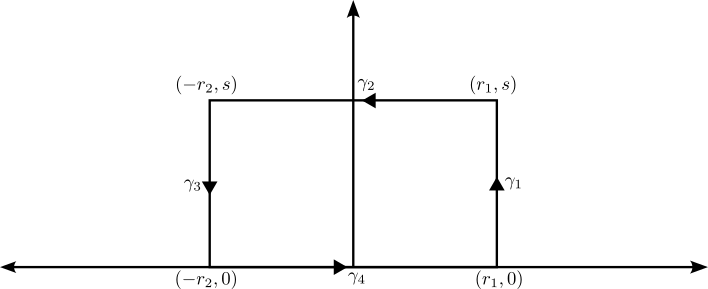
\includegraphics{Images/rational_exp_contour.png}
    \caption{We integrate over the boundary of this rectangle}
    \label{fig:rational-exp-contour}
\end{figure}

Let $C$ be a constant such that
$$ \abs{R(z)} \leq \frac{C}{\abs{z}} $$
Let $\gamma_1$ denote the right side of the rectangle (i.e. the straight path from $(r_1, 0)$ to $(r_1, s)$). Then
\begin{align*}
   \abs{\int_{\gamma_1} R(z) e^{iz} dz} &\leq \int_{\gamma_1} \abs{R(z)} \abs{e^{iz}} dz\\
   &\leq C \int_{\gamma_1} \abs{ \frac{e^{iz}}{z} dz }\\
   &\leq C \int_{0}^s \abs{\frac{e^{i(r_1 + iy)}}{r_1 + iy} idy}\\
   &\leq C \int_{0}^s \frac{e^{-y}}{\sqrt{r_1^2 + y^2}} dy\\
   &\leq \frac{C}{r_1} \int_0^s e^{-y} dy\\
   &= \frac{C}{r_1}(1 - e^{-s})\\
   &< \frac{C}{r_1}
 \end{align*}
Similarly by integrating along the left side of the rectangle, we can conclude that it is less than $\frac{C}{r_2}$. Now we wish to bound the rectangle along the top side of the rectangle. Let $\gamma_2$ denote the straight path from $(r_1, s)$ to $(-r_2, s)$. Then we have 
\begin{align*}
    \abs{\int_{\gamma_2} R(z) e^{iz} dz} &\leq C \int_{\gamma_2} \frac{\abs{e^{i(x + is)}}}{\abs{z}} dz\\
    &\leq Ce^{-s} \int_{-r_2}^{r_1} \frac{1}{\sqrt{x^2 + s^2}} dx\\
    &< Ce^{-s} \int_{-r_2}^{r_1}\frac{1}{s} dx\\
    &= \frac{Ce^{-s}(r_1 + r_2)}{s}
 \end{align*}
 Then we see that as $s \to \infty$ (and we fix $r_1, r_2$), the integral over $\gamma_2$ goes to 0. We know by the residue theorem that integral over the boundary of the rectangle is given by the sum of the residues in the upper half plane (assuming we take $r_1, r_2, s$ sufficiently large). Thus we get
 \begin{align*}
     \abs{\int_{\gamma} R(x) e^{ix} dx -  \int_{-r_2}^{r_1} R(x) e^{ix} dx} &= \abs{\int_{\gamma_1} R(x) e^{ix} dx + \int_{\gamma_2} R(x) e^{ix} dx + \int_{\gamma_3} R(x) e^{ix} dx}\\
     &< \frac{C}{r_1} + \frac{Ce^{-s}(r_1 + r_2)}{s} + \frac{C}{r_2}
 \end{align*}
 Fixing $r_1, r_2$ we can send $s \to \infty$ which removes the middle term. Then by sending $r_1, r_2$ to $\infty$ we conclude that
 $$ \int_{-\infty}^{\infty} R(x) e^{ix} dx = \sum_{\Im(z) > 0} res(R(z)e^{iz}) $$
 Similarly we can evaluate integrals of $R(x)\cos(mx)$ and $R(x)\sin(mx)$ by considering $e^{imx}$ and even $R(x)\cos^m(x)$ and $R(x) \sin^m(x)$ by writing powers of $\sin/\cos$ as a linear combination of $\sin(kx)$ and $\cos(kx)$ for integers $k < m$.\\

 For a concrete example consider
 $$\int_0^{\infty} \frac{\cos(mx)}{x^2 + 1}dx = \frac{1}{2} \int_{-\infty}^{\infty} \frac{\cos(mx)}{x^2 + 1}dx$$
Thus we need to consider the real part of 
$$\int_{-\infty}^{\infty} \frac{e^{imx}}{x^2 + 1} dx$$
Substituting $z = mx$ we get
\begin{align*}
    \int_{-\infty}^{\infty} \frac{e^{imx}}{x^2 + 1}dx &= \frac{1}{m} \int_{-\infty}^{\infty} \frac{e^z}{(z/m)^2 + 1} dz\\
    &= \frac{2\pi i}{m} \sum_{\Im(z) > 0} res \left( \frac{m^2 e^{iz}}{z^2 + m^2} \right)
\end{align*}
The only pole of the function in the upper half-plane if $im$ at which point the residue is $\frac{m^2 e^{-m}}{2im}$. Hence
$$\int_{-\infty}^{\infty} \frac{e^{imx}}{x^2 + 1} dx = \frac{2\pi i}{m} \cdot \frac{m^2 e^{-m}}{2im} = \pi e^{-m} $$
Since this is real we can immediately conclude 
\begin{align*}
    \int_{0}^\infty \frac{\cos(mx)}{x^2 + 1}dx = \frac{\pi e^{-m}}{2}
\end{align*}

\subsection{Poles on the real axis}
There are times when the rational function $R(x)$ has a pole on the real axis but $R(x) \sin x$ or $R(x) \cos(x)$ is still integrable over the real line. A primary example of this is $\frac{\sin x}{x}$. Note in this case our previous contour will not work since a pole lies on the curve itself. In order to avoid this, we go around 0 by including a small semicircle of radius $\delta$ on the contour.
\begin{figure}[h]
    \centering
    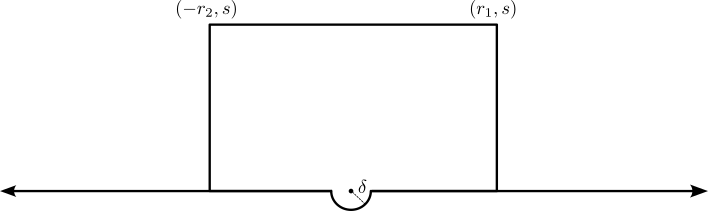
\includegraphics{Images/real_pole_contour.png}
    \caption{We go around the pole at 0}
    \label{fig:real-pole-contour}
\end{figure}

Since $R(z)e^{iz}$ has a simple pole at $0$, we know that $zR(z) e^{iz}$ must be analytic at 0. Thus we can write
$$R(z) e^{iz} = \frac{B}{z} + R_0(z)$$
where $B$ is the residue of $R(z)e^{iz}$ at 0 and $R_0(z)$ is a function that is analytic at 0. Then we see that the integral of the first term over the small semicircle is $\pi i B$ (one can verify this by direct computation if they so desire) and the integral of the second term depends on $\delta$. Therefore it goes to 0 as $\delta \to 0$ (for sufficiently small $\delta$ we can find a local primitive $F$ defined on an open set containing the semicircle. The integral is given by $F(\delta) - F(-\delta)$ which goes to 0 as $\delta$ goes to 0 by continuity of $F$). Hence we conclude that
$$\int_{-\infty}^{\infty} R(x)e^{ix} dx = 2\pi i \sum_{\Im(z) > 0} res(R(z)e^{iz}) + \pi i \sum_{\Im(z) = 0} res(R(z) e^{iz})$$

Let us in fact consider the example
$$\int_{0}^{\infty} \frac{\sin x}{x} dx$$
We see that $z^{-1} e^{iz}$ has no poles in the upper half-plane and only has a simple pole at 0. By considering the Taylor series of $e^{iz}$ and then multiplying it with $z^{-1}$ we can immediately conclude that the residue at 0 is $1$. Therefore
\begin{align*}
    \int_{-\infty}^{\infty} \frac{e^{iz}}{z} dz = \pi i \cdot 1 = \pi i
\end{align*}
Since $\sin x$ corresponds to the imaginary part, we get 
$$ \int_{0}^{\infty} \frac{\sin x}{x} dx = \frac{1}{2} \cdot \pi  = \frac{\pi}{2} $$

\subsection{Fractional powers of $x$}
So far we've been working with fairly well-behave functions but there are times when we wish to integrate functions like $\sqrt{x}$ which are perfectly well-defined on the real line (or the positive real line to be precise) but not so on the complex plane. The problem, of course, is the fact that this is a multivalued functions so we need to be quite careful with how do we things. In fact we will exploit the multivaluedness to find the answer in a rather clever way. 

First we make things precise. Suppose we want to evaluate something of the form
$$\int_0^\infty \frac{R(x)}{x^\alpha} dx$$
for some $0 < \alpha < 1$ where $R(x)$ has no poles on $[0, \infty)$. First we consider a contour as seen below. In order for this integral to converge, $R$ must have a zero of (at least) order 2 at $\infty$ and (at most) a simple pole at 0. 

In order to evaluate this integral we first need to choose a branch of $x^\alpha$ which in turn requires us to choose a domain on which to specify the branch. We will choose our domain to be $\C \setminus [0, \infty)$ (it might seem odd that we have exclude exactly the region we want to integrate over, we will see that this is precisely what allows us to evaluate the integral). Choosing a branch of $x^\alpha$ is equivalent to choosing a branch of $\arg z$ on this domain; we choose $\arg z$ to lie in $(0, 2\pi)$. 
Wit this set up, we can evaluate the given integral in the complex plane over the contour $\Gamma(\epsilon, r)$ as specified in \autoref{fig:keyhole_contour}.

\begin{figure}[h]
    \centering
    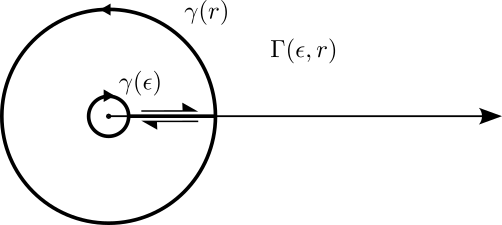
\includegraphics[scale=1.1]{Images/keyhole_contour.png}
    \caption{Contour $\Gamma(\epsilon, r)$ for integrating fractional powers of $x$}
    \label{fig:keyhole_contour}
\end{figure}

In particular, we have a small circle of radius $\epsilon$ called $\gamma(\epsilon)$ and a large circle of radius $r$ which we call $\gamma(r)$. We connect the two circles via the interval on the real line, $[\epsilon, r]$.

Taking $r$ sufficiently large and $\epsilon$ sufficiently small, we can write write
$$ \int_{\Gamma(\epsilon, r)} \frac{R(z)}{z^\alpha} dz = 2\pi i \sum_{\C \setminus [0, \infty)]} res \left( \frac{R(z)}{z^\alpha} \right) $$
We can split in the integral on the left into its separate components 
$$ \int_{\Gamma(\epsilon, r)}  = \int_{\gamma(r)}  + \int_{\gamma(\epsilon)} + \int_{\epsilon}^r  + \int_{r}^\epsilon $$
Under our assumptions for $R$ we know that the integral over $\gamma(r)$ and $\gamma(\epsilon)$ both tend to 0 as $r \to \infty$ and $\epsilon \to 0$. Moreover, after travelling along $\gamma(r)$, $z^\alpha = e^{2\pi i \alpha} \abs{z}^\alpha$. Therefore we conclude 
\begin{align*}
    2\pi i \sum_{\C \setminus [0, \infty)} res \left( \frac{R(z)}{z^\alpha} \right) = \int_0^\infty \frac{R(x)}{x^\alpha} dx - \int_0^\infty e^{-2\pi i \alpha} \frac{R(x)}{x^\alpha} dx = (1 - e^{-2\pi i \alpha}) \int_0^\infty \frac{R(x)}{x^\alpha}dx
\end{align*}

As an example, suppose we want to evaluate
\begin{align*}
    \int_0^\infty \frac{dx}{x^\alpha (1 + x)}
\end{align*}
for $0 < \alpha < 1$. The integrand only has one pole in $\C \setminus [0, \infty)$, at $-1$. By our standard methods for calculating residues (for example we can write $\frac{1}{z^{\alpha}(1 + z)} = \frac{z^{-\alpha}}{1 + z}$ and use \autoref{eg:residue-of-quotient}), we compute that the residue of $1/z^\alpha(1 + z)$ at $-1$ is $(-1)^\alpha = e^{\pi i \alpha}$ (by our choice of $\arg$). Therefore by the above result we get
$$ (1 - e^{-2\pi i \alpha}) \int_0^\infty \frac{dx}{x^\alpha(1 + x)} = 2\pi i \cdot \frac{1}{e^{\pi i \alpha}} $$
Therefore
\begin{align*}
    \int_0^\infty \frac{dx}{x^\alpha(1 + x)} &= \frac{2\pi i}{e^{\pi i \alpha}(1 - e^{-2\pi i \alpha})} = \frac{2\pi i \alpha}{e^{\pi i \alpha} - e^{-\pi i \alpha}} = \frac{2 \pi i \alpha}{2i\sin(\pi \alpha)} = \frac{\pi}{\sin \pi \alpha}
\end{align*}

\subsection{Rational functions and logarithms}
The final example we consider is that of the humble logarithm which is also a multivalued function. So suppose we wish to evaluate
$$ \int_0^\infty R(x) \log(x) dx$$
where $R(x)$ is a rational function with no poles on the non-negative real axis and $xR(x) \to 0$ as $x \to \infty$ (the final condition ensures convergence of the integral). 

We might start by trying something similar to last time. This time what we find is that when the argument of $z$ is $2\pi$ we get $\log(z) = \log(|z|) + 2\pi i$. Once again the integrals over $\gamma(r)$ and $\gamma(\epsilon)$ go to 0 in the limit so we are left with 
$$\int_0^\infty R(x) \log(x) dx - \int_0^\infty R(x) (\log(x) + 2\pi i) dx = 2\pi i \int_0^\infty R(x)dx $$
In particular, the integral we are interested in cancels out. Thus we cannot simply work with $R(x) \log(x)$. Instead what we can do is integrate $R(x) \log(x)^2$. Then we would conclude
\begin{align*}
     2\pi i \sum_{\C \setminus [0, \infty)} res(R(x) \log(x)^2) &= \int_0^\infty R(x) \log(x)^2 dx - \int_0^\infty R(x) (\log(x) + 2\pi i)^2 dx\\
     &= -4\pi i \int_0^\infty R(x) \log(x) dx - (2\pi i)^2 \int_0^\infty R(x) dx 
\end{align*}
We can simplify this to write
$$ \sum_{\C \setminus [0, \infty)} res(R(x) \log(x)^2) = -2 \int_0^\infty R(x) \log(x) dx - 2\pi i \int_0^\infty R(x) dx $$
If $R(x)$ is real-valued then we can equate things by their real and imaginary parts. Finally then, we can say
\begin{align*}
    \int_0^\infty R(x) \log(x) dx &= -\frac{1}{2} \Re\left(\sum_{\C \setminus [0, \infty)} res(R(x) \log(x)^2)\right)\\
    \int_0^\infty R(x) dx &= -\frac{1}{2\pi} \Im\left(\sum_{\C \setminus [0, \infty)} res(R(x) \log(x)^2)\right)
\end{align*}